% Metódy inžinierskej práce

\documentclass[10pt,twoside,slovak,a4paper]{article}

\usepackage[slovak]{babel}
%\usepackage[T1]{fontenc}
\usepackage[IL2]{fontenc} % lepšia sadzba písmena Ľ než v T1
\usepackage[utf8]{inputenc}
\usepackage{graphicx}
\usepackage{url} % príkaz \url na formátovanie URL
\usepackage{hyperref} % odkazy v texte budú aktívne (pri niektorých triedach dokumentov spôsobuje posun textu)

\usepackage{cite}
%\usepackage{times}

%\pagestyle{headings}

\title{Postavy a charaktery v hrách poháňané umelou inteligenciou\thanks{Semestrálny projekt v predmete Metódy inžinierskej práce, ak. rok 2021/22, vedenie: Vladimír Mlynarovič}} % meno a priezvisko vyučujúceho na cvičeniach

\author{Miroslava Mäsiariková\\[2pt]
	{\small Slovenská technická univerzita v Bratislave}\\
	{\small Fakulta informatiky a informačných technológií}\\
	{\small \texttt{xmasiarikova@stuba.sk}}
	}

\date{\small 14. december 2021} % upravte

%\includegraphics[scale=1.0]{diagram.pdf}

\begin{document}

\maketitle

\begin{abstract}

V súčasnosti je umelá inteligencia jeden z hlavných nástrojov na zlepšenie hráčskeho zážitku v hrách. Umelá inteligencia sa v hrách zameriava predovšetkým na tri základné sekcie: schopnosť pohybovať postavami, schopnosť rozhodovať kde a ako sa pohybovať a schopnosť myslieť strategicky. Článok je zameraný  konkrétne na postavy neovládané hráčom, ale umelou inteligenciou. Úlohou týchto postáv je spraviť hru pre hráča ťažšou a zaujímavejšou. Charakter týchto postáv je v hrách rôzny, niektoré majú za úlohu hru iba oživiť a nerobia žiadne špeciálne úkony, zatiaľ čo iné sa samy rozhodujú, pohybujú a skúmajú prostredie okolo seba. Takéto postavy sú schopné učiť sa od ostatných hráčov v hre. V článku je priblížený význam týchto postáv v hrách, ďalej aké algoritmy umelej inteligencie sú potrebné pri modelovaní, správaní a rozhodovaní týchto postáv, s akými problémami sa môžeme stretnúť a ako sa takéto postavy môžu ďalej v hre vyvíjať. 
\end{abstract}

\paragraph{Kľúčové slová:}NPC, non-player character, Finite State Machine, Behaviour Tree, GOAP.

\section{Úvod}

\quad Umelá inteligencia je predovšetkým o vytváraní počítačov, ktoré budú schopné vykonávať úlohy, v ktorých je potrebné používať prirodzené ľudské, alebo zvieracie myslenie. Táto podstata umelej inteligencie je v súčasnosti veľmi skúmanou oblasťou hlavne z pohľadu vývojárov hier, ktorí sa snažia byť pri takomto vývoji čoraz viac kreatívni. A preto vytvárajú algoritmy, s ktorých pomocou postavy v hrách vystupujú alebo konajú ako ľudia či zvieratá. Aktuálnosť tejto témy nám potvrdzuje aj nasledujúca tabuľka ~\ref{t:t1} . V tejto tabuľke sa nachádzajú výsledky z prieskumu, kde sa opýtali 3000 respondentov, ako má podľa nich vyzerať ideálna hra. Až 31\% opýtaných uviedlo, že oceňujú, ak sú v hre NPC, ktoré sa vyvíjajú a tak im hru ďalej komplikujú. 

\begin{table*}[tbh]
\center 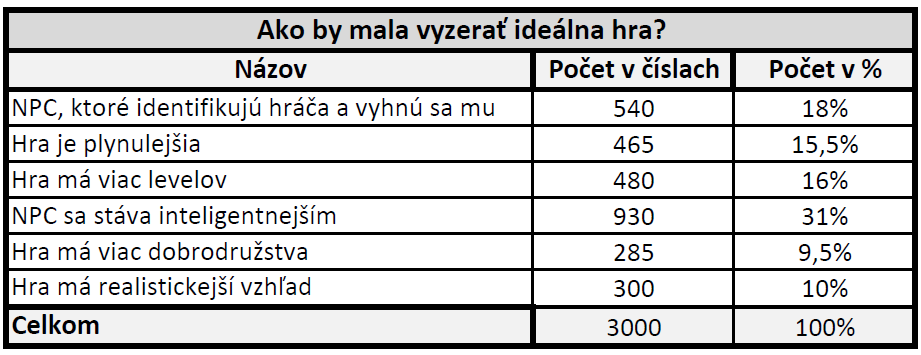
\includegraphics[scale=0.5]{prieskum.png}
\caption{Prieskum o ideálnej hre}
\label{t:t1}
\end{table*}

Hlavným cieľom tohto článku je poukázať práve na túto časť umelej inteligencie a jej využitie v hrách. V druhej kapitole budú predstavené práve také postavy v hrách, ktoré fungujú iba na základe umelej inteligencie a ich využitie. V tretej kapitole sa čitateľ oboznámi s typmi týchto postáv, čím sa od seba líšia a na čo v hrách slúžia. Kapitolu štvrtú tvoria druhy algoritmov, ktoré vývojári hier využívajú pri modelovaní týchto postáv. V poslednej, piatej kapitole je popísaná jednoduchá hra na schovávačku.

Obsah tohto článku vychádza z viacerých odborných článkov či výskumných prác, ktoré boli zhrnuté do jednej ucelenej formy, ktorá poskytne čitateľovi potrebné informácie z tejto aktuálnej problematiky. 


\section{Čo je to NPC a na čo slúži}  \label{nejaka}
\quad NPC \footnote{anglicky non-player character, slovensky postava neovládaná hráčom} slúži na označenie postáv v hrách, ktoré nie sú ovládané hráčom, ale fungujú na základe umelej inteligencie, tzn. ovláda ich sám počítač. Tieto postavy sú nevyhnutnou súčasťou na zatraktívnenie akejkoľvek hry. Ich hlavnou úlohou je spraviť hru pre hráča atraktívnou, zaujímavou a komplikovanejšou, pretože jednoduchá hra pre hráča nie je zaujímavá. 

\quad Charakter týchto postáv by sa dal rozdeliť na dve skupiny, statické a dynamické. V prvej skupine sa nachádzajú postavy, ktorých úlohou je hru iba oživiť a nerobia žiadne špeciálne úlohy. Takéto postavy iba dopĺňajú prostredie, v ktorom sa väčšinou pohybujú po uliciach. Ich správanie v hre je ľahko predvídateľné inými hráčmi, pretože činnosti, ktoré vykonávajú, opakujú stále dookola. V druhej skupine sa nachádzajú postavy, ktoré sú schopné učiť sa od ostatných hráčov v hre, ďalej sa vyvíjať a zlepšovať. Tieto postavy sú schopné samy sa pohybovať, rozhodovať a strategicky myslieť. Ich úlohou je sťažiť reálnym hráčom hru a nedovoliť im len tak jednoducho vyhrať, správanie takýchto postáv je ťažko predvídateľné a často sa mení. Jedinou nevýhodou týchto postáv je, že nie sú ešte dostatočne inteligentné. Väčšina týchto postáv v hrách vedie iba jednoduché dialógy alebo ovplyvňuje priebeh deja na základe doterajších skúseností s hráčmi. 

\quad Jednoduchým príkladom je kartová hra. V takýchto hrách sa okrem hráčov musí nachádzať aj nejaká neutrálna osoba, resp. rozhodca, ktorá bude dozerať na pravidlá hry. Práve touto neutrálnou osobou je postava, ktorá nie je ovládaná žiadnym hráčom, ale počítačom. Tento rozhodca vedie jednoduché dejové dialógy s reálnymi hráčmi, kontroluje dodržiavanie pravidiel a dotvára celkovú atmosféru hry. ~\cite{NPC, AI} 
\begin{figure*}[tbh]
\centering
\end{figure*}
\section{Typy NPC} 
\quad V hernom svete sa môže objaviť niekoľko typov týchto nehrateľných postáv. A to funkčné postavy, opačná kocka, spoluhráči a lídri. 
\begin{itemize}
\item \textbf{Funkčné postavy}

\quad Tieto postavy sú najjednoduchšie z vyššie vymenovaných, pretože nepotrebujú veľkú autonómiu ani inteligenciu. Avšak pokročilejšie postavy z tejto skupiny môžu medzi sebou aj komunikovať prostredníctvom jazyka alebo zadávať či vykonávať rôzne úlohy, aby dosiahli v hre realistickejší efekt. Vďaka umelej inteligencií, ktorú využívajú sa môžu v hre ďalej učiť napríklad prostredníctvom hlasu. Najjednoduchším príkladom je, že ak poviete tejto postave, že jablká sú zelené a pomaranče sú oranžové, tak si to táto postava zapamätá a v jej vedomostiach budú jablká zelené a pomaranče oranžové. Toto bol avšak iba jednoduchý príklad pre pochopenie danej problematiky. V hre je učenie tejto funkčnej postavy skôr o znalostiach potrebných v tomto hráčskom svete, ako napríklad kde kúpiť zbraň, či sa ju oplatí kúpiť, ktorý úkryt je pre ňu vhodný a podobne.  \cite{Types}


\item \textbf{Opačná kocka}

\quad V hrách sa veľmi často stretneme s nejakým šéfom, resp. nepriateľom. Tieto postavy sú vždy riadené práve počítačom. Týchto šéfov môžeme rozdeliť na mini šéfa, super šéfa a finálneho šéfa. Mini šéf nevyužíva veľmi zložitú technológiu umelej inteligencie. Ide iba o obyčajného nepriateľa na základnej úrovni, ktorý sa musí dostať k reálnemu hráčovi dostatočne blízko, v istom časovom intervale a spôsobiť mu nejakú ujmu, aby mu hru skomplikoval. Super šéf je voliteľný nepriateľ pre sťaženie hry a finálny šéf je nepriateľ na konci hry. Super šéf aj finálny šéf sú pre hráča ťažkí nepriatelia, ktorí sa objavia v momente, keď sa môže zdať, že hráč hru vyhrá. Pre tieto postavy je už potrebná pokročilejšia úroveň umelej inteligencie. Pri modelovaní, resp. vývoji, sa hra musí často testovať. Vtedy sa zavolá skupina dobrovoľníkov, ktorých úlohou je objaviť prípadné chyby v hre a predovšetkým vyškoliť nepriateľov, resp. šéfov v hre. Pretože tento nepriateľ sa učí predovšetkým na vlastných chybách a slabinách druhej strany, teda na strane hráča. Vďaka takémuto testovaniu a príprave sa nepriateľ v hre dokáže vyvinúť do takej fázy, aby sa stal čo najmenej poraziteľným.  \cite{Types}

\item \textbf{Spoluhráči}

\quad Postava spoluhráča, ktorú ovláda umelá inteligencia je veľmi ťažko kontrolovateľná, pretože tieto postavy dbajú na spoluprácu medzi sebou. A ak sa nachádza v hre veľa chýb alebo nezrovnalostí, tak tieto postavy nefungujú správne a hra môže dokonca zlyhať. Preto je ťažké nechať umelú inteligenciu vykonávať postavu spoluhráča. V súčasnosti sa tieto postavy ani veľmi v hráčskom prostredí nevyužívajú. Keďže umelá inteligencia funguje aj na hĺbkovom učení je vysoko pravdepodobné, že v budúcnosti budú tieto postavy zlepšovať svoju silu a spoluprácu medzi sebou vďaka ich autonómnemu tréningu. Kedy sa budú postavy učiť bez dozoru a na sebe samých.  \cite{Types}

\item \textbf{Lídri}

\quad Posledným typom neovládateľných postáv sú lídri. Tieto postavy by sa dali prirovnať k súčasnému programu inteligentného robota. Majú totiž svoje samostatné myslenie a učenie. Lídri sa pozerajú na celkovú situáciu v hre, analyzujú zmeny a robia rôzne úsudky. Napríklad v hre s názvom Civilizácia, súťažia hráči práve s takouto postavou a bojujú o územie. Líder sa tu sám rozhoduje na základe aktuálnej situácie, napríklad nadväzuje diplomatické vzťahy, vedie vojny, posiela vojakov do boja, ochraňuje domovy a podobne. Táto časť umelej inteligencie avšak nie je ešte dokonalá a na konci hry sa môže stať, že postava sa bude rozhodovať už iba náhodným výberom.  \cite{Types}

\end{itemize}

\section{Algoritmy umelej inteligencie na modelovanie NPC} 
\quad NPC vznikajú vďaka algoritmom umelej inteligencie, ktorá je v súčasnosti dôležitou súčasťou tvorby zaujímavých hier. V umelej inteligencií existujú tri typy algoritmov, ktoré sa podieľajú na modelovaní NPC. A to Finite State Machine, Behaviour Tree a Goal-Oriented Action Planning.  
\begin{itemize}
\item \textbf{Finite State Machine (FSM)}

\quad FSM \footnote{slovensky Konečný automat} je bežný algoritmus, ktorý sa využíva pri modelovaní NPC. Tento algoritmus pozostáva zo stavov, ktoré obsahujú navzájom súvisiace akcie. Tieto akcie predstavujú činnosti, ktoré bude postava v hre vykonávať. Výhodou FSM pri tomto modelovaní je, že sa stavy ľahko vytvárajú a kontrolujú. Naopak nevýhodou tohto algoritmu je, že zvolená činnosť, ktorú má postava vykonať, bude vždy rovnaká, takže ju môže hráč neskôr veľmi ľahko v hre predvídať. \cite{NPC}


\item \textbf{Behaviour Tree}

\quad Behaviour Tree \footnote{slovensky Strom správania} je algoritmus umelej inteligencie, ktorý môže riadiť alebo kontrolovať každú akciu NPC na základe hierarchie. V tejto hierarchií sa hlavná zadaná akcia pre NPC zjednoduší na niekoľko menších akcií, čím sa zníži zložitosť týchto zadaných akcií. Behaviour Tree má niekoľko výhod, ktoré môžu zjednodušiť pridelené akcie pre NPC a zároveň sťažiť predvídanie týchto akcií hráčom, čím bude pre nich hra zaujímavejšia.   \cite{NPC}

\item \textbf{Goal-Oriented Action Planning (GOAP)}

\quad GOAP \footnote{voľný preklad do slovenčiny Plánovanie akcie zameranej na cieľ} je algoritmus, v ktorom je NPC voľná pri príprave každej akcie na splnenie stanovených cieľov, tzn. rozhoduje sa sama. Vďaka tomuto algoritmu je NPC v hre dynamickejšia, čo znamená, že jej akcie sa dajú len ťažko predpovedať, a tým je hra pre hráča zaujímavejšia. GOAP pozostáva zo štyroch komponentov, a to z cieľa, akcie, plánu a formulácie plánu. Cieľ predstavuje hlavnú úlohu NPC, ktorú musí táto postava dosiahnuť, akcia predstavuje správanie NPC pri dosahovaní cieľa, plán predstavuje usporiadanie akcií zameraných na vyriešenie cieľa a formulácia plánu predstavuje proces prípravy plánu, ktorý je vhodný pre daný cieľ.  Výhodou používania GOAP pri modelovaní týchto postáv je, že nevytvára zložité grafy na plánovanie. Ďalšou z výhod použitia GOAP pre vývojárov je, že vytvára uzly získané z akcií so vstupom a výstupom, ktoré je možné vyhodnocovať v reálnom čase. Diagram~\ref{f:d1} nižšie zobrazuje stratégiu NPC v hre na schovávanie pomocou algoritmu GOAP.  \cite{NPC}
\begin{figure*}[tbh]
\center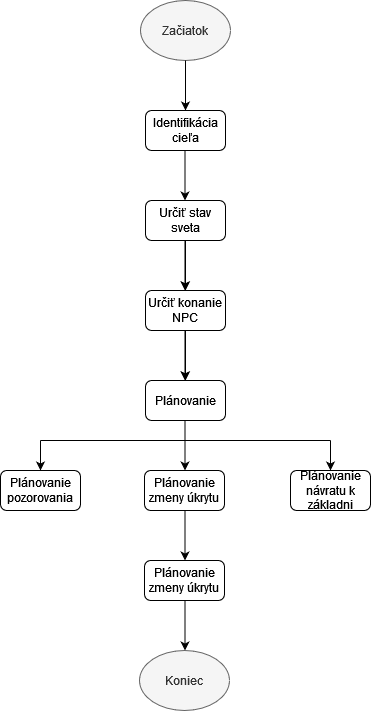
\includegraphics[scale=0.5]{diagram1.png}
\caption{GOAP algoritmus v hre na skrývanie}
\label{f:d1}
\end{figure*}
\end{itemize}

\section{Príklad: Skrývanie} 
\quad NPC majú v hrách rôzne úlohy a jednou z nich je aj skrývanie. Je veľa spôsobov, akými môže byť stratégia skrývania v hre využitá. Môže ísť o doplnok, ktorý má hru iba oživiť alebo môže ísť o hru samotnú. Jedná sa o hru na schovávačku, ktorá je tu už dlho a je pravdepodobne každému známa. Táto hra je veľmi jednoduchá a vyžaduje iba dvoch hráčov, jedného ako pátrača a druhého ako skrytú osobu. Hra začne od hľadača resp. pátrača v základni, kde bude so zavretými očami odpočítavať od vopred určeného čísla po nulu. Hra pokračuje po tom, čo pátrač dokončí odpočítavanie. Úlohou pátrača je hľadať nepriateľa, ktorý sa niekde skrýva a zároveň dohliadať na základňu. Ak pátrač nájde nepriateľov úkryt, nepriateľ aj pátrač sa rozbehnú na základňu. Ak pátrač dorazí na základňu prvý, tak ďalším hľadajúcim sa stane nepriateľ, v opačnom prípade je nepriateľ v bezpečí. Pátrač bude pokračovať v hľadaní nepriateľov, kým ich všetkých nezajme alebo kým nebudú všetci v bezpečí. Ak pátrač chytí všetkých nepriateľov, hra sa skončí a pokračuje na ďalšiu ťažšiu úroveň. Ide o veľmi jednoduchú digitálnu hru, kde NPC predstavuje nepriateľa, čiže postavu, ktorá sa musí schovať a reálny hráč je pátračom. V takejto hre NPC musí zvažovať zmenu miesta na bezpečnejšie a tiež to, ako konať v prípade, ak ho nájde pátrač. NPC tak musí vykonávať niekoľko akcií, ktoré sú zobrazené aj v diagrame~\ref{f:d1} . Diagram ~\ref{f:d2} nižšie zobrazuje priebeh tejto hry na schovávačku. V tabuľke~\ref{t:t2} sa nachádza miera úspešnosti NPC v takejto hre. Hodnoty sú vypočítané ako podiel NPC, ktoré sa dostali na základňu bez toho aby ich hráč chytil a celkovo nájdených NPC hráčom.
\begin{figure*}[tbh]
\center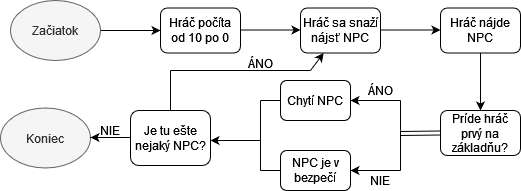
\includegraphics[scale=0.5]{diagram2.png}
\caption{Priebeh hry na skrývanie}
\label{f:d2}
\end{figure*}
\begin{table*}[tbh]
\center 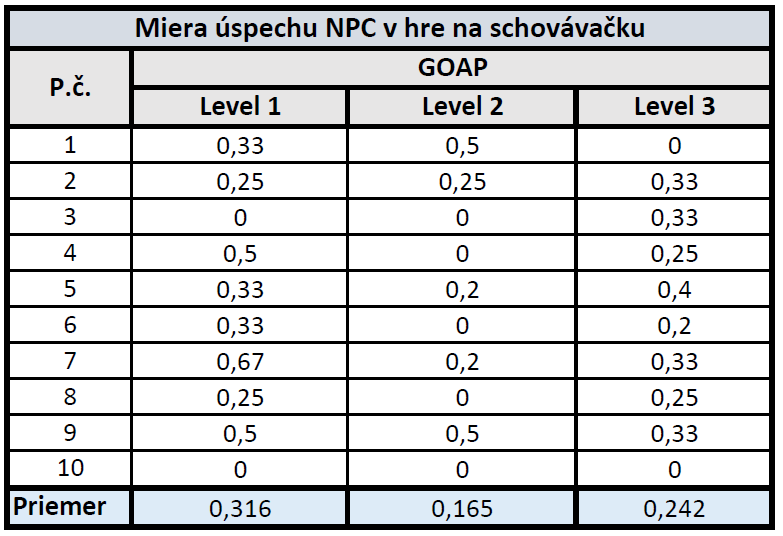
\includegraphics[scale=0.5]{priklad.png}
\caption{Miera úspešnosti NPC v hre na skrývanie}
\label{t:t2}
\end{table*}

\begin{itemize}
\section{Reakcia na témy z prednášok} 
\item \textbf{Inžinierska práca v informatike a písanie technického textu}

\quad Táto prednáška nám mala z môjho pohľadu bližšie priblížiť a predstaviť pojmy ako, kto je to inžinier, čo je to inžinierska práca a ako písať technický text. Tieto témy aj úzko súvisia s vyššie písaným článkom. Z môjho pohľadu bola prednáška veľmi poučná a témy aktuálne. Z tejto prednášky som si odniesla veľa cenných informácií, ktoré mi pomohli pri písaní článku, ale pomôžu mi aj v budúcnosti pri písaní iných odborných prác. Dozvedela som sa, že je dôležité najprv mojej téme, ktorú som si vybrala, dôkladne porozumieť a až potom sa ju snažiť interpretovať v článku. Ďalej som si odniesla poučenie, že pri písaní článkov či rôznych iných technických textov musím byť kreatívna, trpezlivá, a že články by mali byť v prvom rade zmysluplné a obsahovať podložené fakty. Všetky tieto poučenia a informácie som sa snažila aplikovať aj v tomto článku.


\item \textbf{Grafické vyjadrenie informácií v informatike }

\quad Táto prednáška tiež úzko súvisela s písaním odborných prác. Z tejto prednášky som si odniesla poznatky o tom, že článok by mal byť interpretovaný aj vizuálne. To znamená, neobsahovať len odborné fakty, ale mal by aj odborne vyzerať. A preto som sa snažila aj v tomto článku niektoré informácie podať graficky, napríklad pomocou diagramov či tabuliek. Týmito rôznymi grafickými pomôckami sa mi tak podarilo text sprehľadniť a lepšie tak zároveň znázorniť niektoré informácie. Z prednášky som sa ďalej dozvedela, že diagramy pre nás ako pre informatikov sú veľmi dôležité, a že v budúcnosti ich budeme ešte veľa využívať, a preto bolo dobre vyskúšať si už teraz takúto prácu s nimi.

\item \textbf{Prezentácia: slajdy a prednes }

\quad V rámci tejto prednášky nám boli prednesené informácie ako by mala vyzerať odborná prezentácia a prednes k nej. Táto prednáška bola taktiež veľmi užitočná, nakoľko som prezentáciu vypracovala aj k tomuto článku. Poznatky, ktoré som si z tejto prednášky odniesla som implementovala aj do mojej prezentácie a prednesu, ktorý som k nej mala. V rámci mojej prezentácie som sa snažila dodržať štruktúru slajdov, ktorá nám bola prednesená na tejto prednáške, taktiež som sa snažila mať k nej pútavý a zmysluplný prednes a dodržať stanovený čas. Na prednáške som sa zoznámila aj s inými nástrojmi, ktoré mi môžu v budúcnosti pomôcť pri vypracovávaní prezentácií, aby boli stále niečím zaujímavé a pútavé.

\item \textbf{Vedecké publikovanie v informatike. Plagiátorstvo a ako sa mu vyhnúť}

\quad Táto prednáška sa niesla v duchu plagiátorstva. Nakoľko ako informatici či inžinieri budeme často písať rôzne práce, či už počas štúdia alebo nášho pracovného života, je z môjho pohľadu dôležité vedieť informácie správne aplikovať do týchto prác. A v podobnej myšlienke sa niesla aj táto prednáška, ktorá plynule nadväzovala na tie predchádzajúce. Na začiatku prednášky som sa oboznámila s tým, že ak chcem písať nejakú prácu je dôležité jej najprv celkovo porozumieť a preskúmať danú problematiku. Ďalej som sa dozvedela, že takáto práca musí byť celistvá, vychádzať iba z faktov a nesmie obsahovať zbytočnosti. Taktiež som si z tejto prednášky odniesla, že je dôležité najprv preštudovať viacero rôznych zdrojov a až potom začať písať nejakú prácu. Tento spôsob som vyskúšala aj na tomto článku, kde som si najprv preštudovala niekoľko zaujímavých článkov, z ktorých som si spísala štruktúru a vybrala dôležité myšlienky, a až potom som začala písať tento článok. Samozrejme aj popri článku som hľadala ďalšie zdroje, ktoré som sa snažila v článku využiť. Hlavnou témou tejto prednášky bolo teda plagiátorstvo, bolo nám vysvetlené ako vzniká, ako sa mu vyhnúť a aké následky nás čakajú ak plagiátorstvo spáchame. Z tejto témy som sa taktiež poučila a preto som v článku označila všetky zdroje, z ktorých som čerpala informácie.  

\end{itemize}

\section{Záver} \label{zaver} 
\quad S rýchlym vývojom dnešných technológií dochádza k veľkým prelomom najmä v oblasti umelej inteligencie, ktorá v sebe nesie veľký potenciál. Čoskoro sa stane nenahraditeľnou súčasťou pre vývoj všetkých hier. Ako bolo prezentované aj v tomto článku, umelá inteligencia je najlepším spôsobom pre inteligentný vývoj NPC v hrách. V súčasnosti môže herná umelá inteligencia plniť úlohy zadané vývojárom a vytvárať tak realistickú ilúziu „skutočných postáv“. A to na základe toho, že sa učí na tom, ako sa správajú reálni hráči alebo ako medzi sebou komunikujú. Môj názor je, že NPC prinesie v budúcnosti herným spoločnostiam obrovské zisky a poskytne nový smer pre herný priemysel. Taktiež strojové učenie je základným nástrojom na získavanie údajov pre analýzu hier, takže herné spoločnosti môžu študovať správanie hráčov a dešifrovať tak nové poznatky na zlepšenie svojich hier v priebehu krátkeho času. Čo sa týka samoučiacej sa funkcie umelej inteligencie, tak sa jedná stále pomerne o novinku, ale časom, po tom čo sa vo vývoji hier začnú využívať nové a vylepšené verzie umelej inteligencie, ktoré budú založené na strojovom učení, bude budúci vývoj hier, hrateľnosť a celkový herný zážitok nakoniec lepší a modernejší.

%\footnote{Niekedy môžete potrebovať aj poznámku pod čiarou.}



%\acknowledgement{Ak niekomu chcete poďakovať\ldots}


% týmto sa generuje zoznam literatúry z obsahu súboru literatura.bib podľa toho, na čo sa v článku odkazujete
\bibliography{literatura}
\bibliographystyle{plain} % prípadne alpha, abbrv alebo hociktorý iný
\end{document}
